\documentclass{beamer}

\usepackage[utf8]{inputenc}
\usepackage{hyperref}
\usepackage{lmodern}
\usefonttheme{professionalfonts}
\usepackage{amssymb, amsmath}
\usepackage [lambda,
advantage,
operators,
sets,
adversary,
landau,
probability,
notions,
logic,
ff,
mm,
primitives,
events,
complexity,
asymptotics,
keys]{ cryptocode }

\usepackage{tikz}
\usetikzlibrary{arrows}


%Information to be included in the title page:
\title{Lossy Trapdoor Functions}
\author{Giacomo Fenzi}
\institute{ETH Zurich}
\date{22 April 2021}



\begin{document}

\frame{\titlepage}

\begin{frame}
    \frametitle{Motivation}
    \begin{itemize}
        \item Trapdoor Functions are basic primitive, but hard to instantiate
        \item CCA Security from factoring and discrete log but not lattices
    \end{itemize}


\end{frame}


\begin{frame}
    \frametitle{Results}
    \begin{itemize}
        \item Introduce Lossy Trapdoor Functions (LTDFs)
        \item Realize LTDFs from factoring, discrete log \textit{and} lattices
        \item Show LDTFs imply TDFs
        \item Black box construction of CCA-secure (witness recovering) cryptosystems,
              collision-resistant hash functions and oblivious transfer protocols.
    \end{itemize}

\end{frame}

\begin{frame}
    \frametitle{Connections}
    \begin{center}
        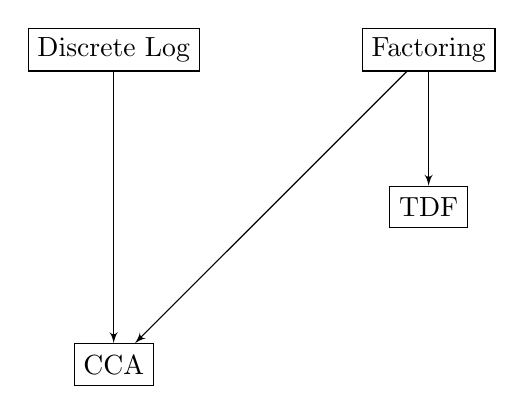
\begin{tikzpicture}
            \tikzset{vertex/.style = {shape=rectangle,draw,minimum size=1.5em}}
            \tikzset{edge/.style = {->,> = latex'}}
            \node[vertex] (a) at  (0,0) {Discrete Log};
            \node[vertex] (b) at  (4,0) {Factoring};
            \node[vertex] (c) at  (0, -4) {CCA};
            \node[vertex] (d) at  (4, -2) {TDF};

            \draw[edge] (b) to (d);
            \draw[edge] (b) to (c);
            \draw[edge] (a) to (c);
        \end{tikzpicture}
    \end{center}
\end{frame}


\begin{frame}
    \frametitle{Connections}
    \begin{center}
        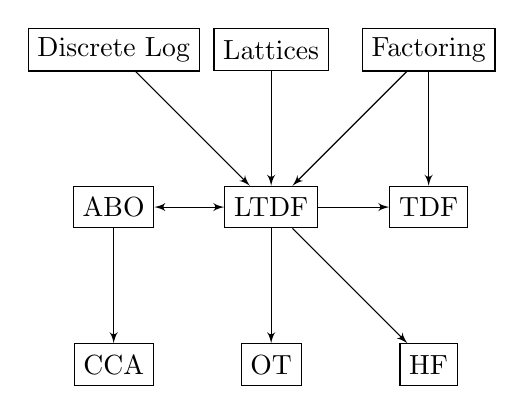
\begin{tikzpicture}
            \tikzset{vertex/.style = {shape=rectangle,draw,minimum size=1.5em}}
            \tikzset{edge/.style = {->,> = latex'}}
            \node[vertex] (a) at  (0,0) {Discrete Log};
            \node[vertex] (j) at  (2,0) {Lattices};
            \node[vertex] (b) at  (4,0) {Factoring};
            \node[vertex] (c) at  (0, -4) {CCA};
            \node[vertex] (d) at  (4, -2) {TDF};
            \node[vertex] (e) at  (2, -2) {LTDF};
            \node[vertex] (f) at  (0, -2) {ABO};
            \node[vertex] (g) at  (2, -4) {OT};
            \node[vertex] (h) at  (4, -4) {HF};

            \draw[edge] (b) to (d);
            \draw[edge] (b) to (e);
            \draw[edge] (a) to (e);
            \draw[edge] (f) to (c);
            \draw[edge] (e) to (d);
            \draw[edge, <->] (e) to (f);
            \draw[edge] (e) to (g);
            \draw[edge] (e) to (h);
            \draw[edge] (j) to (e);
        \end{tikzpicture}
    \end{center}
\end{frame}

\begin{frame}
    \frametitle{Notation and Entropy}
    \begin{itemize}
        \item $\secpar$ is the security parameter, and
              we will abbreviate $n(\secpar) = \poly$ as simply $n$
    \end{itemize}
\end{frame}

\begin{frame}
    \frametitle{Trapdoor Functions}
    Informally, a trapdoor function is family of functions that are
    hard to invert without access to some additional information called a trapdoor
    \begin{definition}
        A trapdoor function consists of three PPT algorithms $(S, F, F^{-1})$
        such that:
        \begin{itemize}
            \item \textit{Easy to sample and invert with trapdoor.} $S(\secparam) \rightarrow (s, t)$
                  such that $F(s, {-})$ is an injective function on $\bin^n$ and $F^{-1}(t, {-})$ is its inverse
            \item \textit{Hard to invert without.} For \textit{any} PPT inverter $\adv$ we have that $\adv(\secparam, s, F(s, x))$
                  outputs $x$ with negligible probability.
        \end{itemize}
    \end{definition}
\end{frame}

\begin{frame}
    \frametitle{Example of Trapdoor}
    RSA Encryption! In trapdoor form:
    \begin{itemize}
        \item $S(\secparam)$ generates $N, e, d$ as in RSA,
              set $s = (N, e)$ and $t = (d)$ and returns $(s, t)$
        \item $F(s, x)$ computes $x^e \mod N$
        \item $F^{-1}(t, c)$ computes $c^d \mod N$
    \end{itemize}
\end{frame}


\end{document}